\chapter{Độ phức tạp thời gian}

\index{time complexity}

Hiệu quả của các thuật toán là rất quan trọng trong lập trình thi đấu.
Thông thường, việc thiết kế một thuật toán
giải quyết bài toán một cách chậm chạp là dễ dàng,
nhưng thách thức thực sự là phát minh ra một
thuật toán nhanh.
Nếu thuật toán quá chậm, nó sẽ chỉ nhận được điểm một phần hoặc không có điểm nào cả.

\key{Độ phức tạp thời gian (time complexity)} của một thuật toán
ước tính thời gian mà thuật toán sẽ sử dụng
cho một đầu vào nào đó.
Ý tưởng là biểu diễn hiệu quả
dưới dạng một hàm có tham số là kích thước của đầu vào.
Bằng cách tính toán độ phức tạp thời gian,
chúng ta có thể biết được thuật toán có đủ nhanh hay không
mà không cần phải triển khai nó.

\section{Quy tắc tính toán}

Độ phức tạp thời gian của một thuật toán
được ký hiệu là $O(\cdots)$
trong đó ba dấu chấm đại diện cho một
hàm nào đó.
Thông thường, biến $n$ biểu thị
kích thước đầu vào.
Ví dụ, nếu đầu vào là một mảng các số,
$n$ sẽ là kích thước của mảng,
và nếu đầu vào là một chuỗi,
$n$ sẽ là độ dài của chuỗi.

\subsubsection*{Vòng lặp}

Một lý do phổ biến khiến một thuật toán bị chậm là
nó chứa nhiều vòng lặp duyệt qua đầu vào.
Thuật toán càng chứa nhiều vòng lặp lồng nhau,
nó càng chậm.
Nếu có $k$ vòng lặp lồng nhau,
độ phức tạp thời gian là $O(n^k)$.

Ví dụ, độ phức tạp thời gian của đoạn mã sau là $O(n)$:
\begin{lstlisting}
for (int i = 1; i <= n; i++) {
    // code
}
\end{lstlisting}

Và độ phức tạp thời gian của đoạn mã sau là $O(n^2)$:
\begin{lstlisting}
for (int i = 1; i <= n; i++) {
    for (int j = 1; j <= n; j++) {
        // code
    }
}
\end{lstlisting}

\subsubsection*{Bậc độ lớn}

Một độ phức tạp thời gian không cho chúng ta biết số lần chính xác
mà đoạn mã bên trong một vòng lặp được thực thi,
mà nó chỉ cho thấy bậc độ lớn.
Trong các ví dụ sau, đoạn mã bên trong vòng lặp
được thực thi $3n$, $n+5$ và $\lceil n/2 \rceil$ lần,
nhưng độ phức tạp thời gian của mỗi đoạn mã là $O(n)$.

\begin{lstlisting}
for (int i = 1; i <= 3*n; i++) {
    // code
}
\end{lstlisting}

\begin{lstlisting}
for (int i = 1; i <= n+5; i++) {
    // code
}
\end{lstlisting}

\begin{lstlisting}
for (int i = 1; i <= n; i += 2) {
    // code
}
\end{lstlisting}

Một ví dụ khác,
độ phức tạp thời gian của đoạn mã sau là $O(n^2)$:

\begin{lstlisting}
for (int i = 1; i <= n; i++) {
    for (int j = i+1; j <= n; j++) {
        // code
    }
}
\end{lstlisting}

\subsubsection*{Các giai đoạn}

Nếu thuật toán bao gồm các giai đoạn liên tiếp,
tổng độ phức tạp thời gian là độ phức tạp thời gian lớn nhất
của một giai đoạn đơn lẻ.
Lý do cho điều này là giai đoạn chậm nhất
thường là nút thắt cổ chai của đoạn mã.

Ví dụ, đoạn mã sau bao gồm
ba giai đoạn với các độ phức tạp thời gian
$O(n)$, $O(n^2)$ và $O(n)$.
Do đó, tổng độ phức tạp thời gian là $O(n^2)$.

\begin{lstlisting}
for (int i = 1; i <= n; i++) {
    // code
}
for (int i = 1; i <= n; i++) {
    for (int j = 1; j <= n; j++) {
        // code
    }
}
for (int i = 1; i <= n; i++) {
    // code
}
\end{lstlisting}

\subsubsection*{Nhiều biến số}

Đôi khi độ phức tạp thời gian phụ thuộc vào
nhiều yếu tố.
Trong trường hợp này, công thức độ phức tạp thời gian
chứa nhiều biến.

Ví dụ, độ phức tạp thời gian của
đoạn mã sau là $O(nm)$:

\begin{lstlisting}
for (int i = 1; i <= n; i++) {
    for (int j = 1; j <= m; j++) {
        // code
    }
}
\end{lstlisting}

\subsubsection*{Đệ quy}

Độ phức tạp thời gian của một hàm đệ quy
phụ thuộc vào số lần hàm được gọi
và độ phức tạp thời gian của một lần gọi.
Tổng độ phức tạp thời gian là tích của
các giá trị này.

Ví dụ, xem xét hàm sau:
\begin{lstlisting}
void f(int n) {
    if (n == 1) return;
    f(n-1);
}
\end{lstlisting}
Lệnh gọi $\texttt{f}(n)$ gây ra $n$ lần gọi hàm,
và độ phức tạp thời gian của mỗi lần gọi là $O(1)$.
Do đó, tổng độ phức tạp thời gian là $O(n)$.

Một ví dụ khác, xem xét hàm sau:
\begin{lstlisting}
void g(int n) {
    if (n == 1) return;
    g(n-1);
    g(n-1);
}
\end{lstlisting}
Trong trường hợp này, mỗi lần gọi hàm tạo ra hai
lần gọi khác, ngoại trừ $n=1$.
Hãy xem điều gì xảy ra khi $g$ được gọi
với tham số $n$.
Bảng sau cho thấy các lần gọi hàm
được tạo ra bởi một lệnh gọi này:
\begin{center}
\begin{tabular}{rr}
lệnh gọi hàm & số lần gọi \\
\hline
$g(n)$ & 1 \\
$g(n-1)$ & 2 \\
$g(n-2)$ & 4 \\
$\cdots$ & $\cdots$ \\
$g(1)$ & $2^{n-1}$ \\
\end{tabular}
\end{center}
Dựa trên điều này, độ phức tạp thời gian là
\[1+2+4+\cdots+2^{n-1} = 2^n-1 = O(2^n).\]

\section{Các lớp độ phức tạp}

\index{complexity classes}

Danh sách sau đây chứa các độ phức tạp thời gian phổ biến
của các thuật toán:

\begin{description}
\item[$O(1)$]
\index{constant-time algorithm}
Thời gian chạy của một thuật toán \key{thời gian hằng số}
không phụ thuộc vào kích thước đầu vào.
Một thuật toán thời gian hằng số điển hình là một
công thức trực tiếp tính toán câu trả lời.

\item[$O(\log n)$]
\index{logarithmic algorithm}
Một thuật toán \key{logarit} thường
giảm một nửa kích thước đầu vào ở mỗi bước.
Thời gian chạy của một thuật toán như vậy
là logarit, bởi vì
$\log_2 n$ bằng số lần
$n$ phải được chia cho 2 để được 1.

\item[$O(\sqrt n)$]
Một thuật toán \key{căn bậc hai} chậm hơn
$O(\log n)$ nhưng nhanh hơn $O(n)$.
Một thuộc tính đặc biệt của căn bậc hai là
$\sqrt n = n/\sqrt n$, vì vậy căn bậc hai $\sqrt n$ nằm,
theo một nghĩa nào đó, ở giữa đầu vào.

\item[$O(n)$]
\index{linear algorithm}
Một thuật toán \key{tuyến tính} duyệt qua đầu vào
một số lần không đổi.
Đây thường là độ phức tạp thời gian tốt nhất có thể,
bởi vì thường cần phải truy cập từng
phần tử đầu vào ít nhất một lần trước khi
báo cáo câu trả lời.

\item[$O(n \log n)$]
Độ phức tạp thời gian này thường chỉ ra rằng
thuật toán sắp xếp đầu vào,
bởi vì độ phức tạp thời gian của các thuật toán
sắp xếp hiệu quả là $O(n \log n)$.
Một khả năng khác là thuật toán
sử dụng một cấu trúc dữ liệu trong đó mỗi thao tác
mất thời gian $O(\log n)$.

\item[$O(n^2)$]
\index{quadratic algorithm}
Một thuật toán \key{bậc hai} thường chứa
hai vòng lặp lồng nhau.
Có thể duyệt qua tất cả các cặp
phần tử đầu vào trong thời gian $O(n^2)$.

\item[$O(n^3)$]
\index{cubic algorithm}
Một thuật toán \key{bậc ba} thường chứa
ba vòng lặp lồng nhau.
Có thể duyệt qua tất cả các bộ ba
phần tử đầu vào trong thời gian $O(n^3)$.

\item[$O(2^n)$]
Độ phức tạp thời gian này thường chỉ ra rằng
thuật toán lặp qua tất cả các
tập hợp con của các phần tử đầu vào.
Ví dụ, các tập hợp con của $\{1,2,3\}$ là
$\emptyset$, $\{1\}$, $\{2\}$, $\{3\}$, $\{1,2\}$,
$\{1,3\}$, $\{2,3\}$ và $\{1,2,3\}$.

\item[$O(n!)$]
Độ phức tạp thời gian này thường chỉ ra rằng
thuật toán lặp qua tất cả các
hoán vị của các phần tử đầu vào.
Ví dụ, các hoán vị của $\{1,2,3\}$ là
$(1,2,3)$, $(1,3,2)$, $(2,1,3)$, $(2,3,1)$,
$(3,1,2)$ và $(3,2,1)$.

\end{description}

\index{polynomial algorithm}
Một thuật toán là \key{đa thức}
nếu độ phức tạp thời gian của nó nhiều nhất là $O(n^k)$
trong đó $k$ là một hằng số.
Tất cả các độ phức tạp thời gian trên ngoại trừ
$O(2^n)$ và $O(n!)$ là đa thức.
Trong thực tế, hằng số $k$ thường nhỏ,
và do đó, một độ phức tạp thời gian đa thức
có nghĩa gần đúng là thuật toán đó \emph{hiệu quả}.

\index{NP-hard problem}

Hầu hết các thuật toán trong cuốn sách này là đa thức.
Tuy nhiên, có nhiều bài toán quan trọng mà
không có thuật toán đa thức nào được biết đến, tức là,
không ai biết cách giải quyết chúng một cách hiệu quả.
Các bài toán \key{NP-khó} là một tập hợp quan trọng
các bài toán mà không có thuật toán đa thức nào
được biết đến\footnote{Một cuốn sách kinh điển về chủ đề này là
cuốn \emph{Computers and Intractability: A Guide to the Theory
of NP-Completeness} của M. R. Garey và D. S. Johnson \cite{gar79}.}.

\section{Ước tính hiệu quả}

Bằng cách tính toán độ phức tạp thời gian của một thuật toán,
có thể kiểm tra, trước khi
triển khai thuật toán, rằng nó
đủ hiệu quả cho bài toán.
Điểm khởi đầu cho các ước tính là thực tế rằng
một máy tính hiện đại có thể thực hiện khoảng vài trăm
triệu phép toán trong một giây.

Ví dụ, giả sử giới hạn thời gian cho
một bài toán là một giây và kích thước đầu vào là $n=10^5$.
Nếu độ phức tạp thời gian là $O(n^2)$,
thuật toán sẽ thực hiện khoảng $(10^5)^2=10^{10}$ phép toán.
Việc này sẽ mất ít nhất vài chục giây,
vì vậy thuật toán có vẻ quá chậm để giải quyết bài toán.

Mặt khác, với kích thước đầu vào cho trước,
chúng ta có thể thử \emph{đoán}
độ phức tạp thời gian cần thiết của thuật toán
để giải quyết bài toán.
Bảng sau đây chứa một số ước tính hữu ích
giả sử giới hạn thời gian là một giây.

\begin{center}
\begin{tabular}{ll}
kích thước đầu vào & độ phức tạp thời gian yêu cầu \\
\hline
$n \le 10$ & $O(n!)$ \\
$n \le 20$ & $O(2^n)$ \\
$n \le 500$ & $O(n^3)$ \\
$n \le 5000$ & $O(n^2)$ \\
$n \le 10^6$ & $O(n \log n)$ hoặc $O(n)$ \\
$n$ lớn & $O(1)$ hoặc $O(\log n)$ \\
\end{tabular}
\end{center}

Ví dụ, nếu kích thước đầu vào là $n=10^5$,
có lẽ người ta mong đợi rằng độ phức tạp
thời gian của thuật toán là $O(n)$ hoặc $O(n \log n)$.
Thông tin này giúp việc thiết kế thuật toán dễ dàng hơn,
bởi vì nó loại bỏ các phương pháp tiếp cận sẽ mang lại
một thuật toán có độ phức tạp thời gian tồi tệ hơn.

\index{constant factor}

Tuy nhiên, điều quan trọng cần nhớ là
độ phức tạp thời gian chỉ là một ước tính về hiệu quả,
bởi vì nó ẩn đi các \emph{hệ số hằng}.
Ví dụ, một thuật toán chạy trong thời gian $O(n)$
có thể thực hiện $n/2$ hoặc $5n$ phép toán.
Điều này có ảnh hưởng quan trọng đến thời gian
chạy thực tế của thuật toán.

\section{Tổng con lớn nhất}

\index{maximum subarray sum}

Thường có nhiều thuật toán khả dĩ
để giải quyết một bài toán sao cho
độ phức tạp thời gian của chúng khác nhau.
Phần này thảo luận về một bài toán kinh điển
có một giải pháp $O(n^3)$ đơn giản.
Tuy nhiên, bằng cách thiết kế một thuật toán tốt hơn,
có thể giải quyết bài toán trong thời gian $O(n^2)$
và thậm chí trong thời gian $O(n)$.

Cho một mảng gồm $n$ số,
nhiệm vụ của chúng ta là tính toán
\key{tổng con lớn nhất (maximum subarray sum)}, tức là,
tổng lớn nhất có thể của
một dãy các giá trị liên tiếp
trong mảng\footnote{Cuốn sách
\emph{Programming Pearls} của J. Bentley \cite{ben86} đã làm cho bài toán này trở nên phổ biến.}.
Bài toán này thú vị khi có thể có
các giá trị âm trong mảng.
Ví dụ, trong mảng
\begin{center}
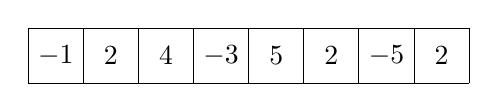
\begin{tikzpicture}[scale=0.7]
\draw (0,0) grid (8,1);

\node at (0.5,0.5) {$-1$};
\node at (1.5,0.5) {$2$};
\node at (2.5,0.5) {$4$};
\node at (3.5,0.5) {$-3$};
\node at (4.5,0.5) {$5$};
\node at (5.5,0.5) {$2$};
\node at (6.5,0.5) {$-5$};
\node at (7.5,0.5) {$2$};
\end{tikzpicture}
\end{center}
\begin{samepage}
mảng con sau đây tạo ra tổng lớn nhất là $10$:
\begin{center}
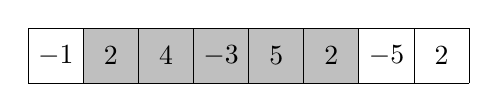
\begin{tikzpicture}[scale=0.7]
\fill[color=lightgray] (1,0) rectangle (6,1);
\draw (0,0) grid (8,1);

\node at (0.5,0.5) {$-1$};
\node at (1.5,0.5) {$2$};
\node at (2.5,0.5) {$4$};
\node at (3.5,0.5) {$-3$};
\node at (4.5,0.5) {$5$};
\node at (5.5,0.5) {$2$};
\node at (6.5,0.5) {$-5$};
\node at (7.5,0.5) {$2$};
\end{tikzpicture}
\end{center}
\end{samepage}

Chúng ta giả định rằng một mảng con rỗng được cho phép,
vì vậy tổng con lớn nhất luôn ít nhất là $0$.

\subsubsection{Thuật toán 1}

Một cách đơn giản để giải quyết bài toán
là duyệt qua tất cả các mảng con có thể,
tính tổng các giá trị trong mỗi mảng con và duy trì
tổng lớn nhất.
Đoạn mã sau đây triển khai thuật toán này:

\begin{lstlisting}
int best = 0;
for (int a = 0; a < n; a++) {
    for (int b = a; b < n; b++) {
        int sum = 0;
        for (int k = a; k <= b; k++) {
            sum += array[k];
        }
        best = max(best,sum);
    }
}
cout << best << "\n";
\end{lstlisting}

Các biến \texttt{a} và \texttt{b} xác định chỉ số đầu và
cuối của mảng con,
và tổng các giá trị được tính vào biến \texttt{sum}.
Biến \texttt{best} chứa tổng lớn nhất được tìm thấy trong quá trình tìm kiếm.

Độ phức tạp thời gian của thuật toán là $O(n^3)$,
bởi vì nó bao gồm ba vòng lặp lồng nhau
duyệt qua đầu vào.

\subsubsection{Thuật toán 2}

Dễ dàng làm cho Thuật toán 1 hiệu quả hơn
bằng cách loại bỏ một vòng lặp khỏi nó.
Điều này có thể thực hiện được bằng cách tính tổng tại cùng
thời điểm khi đầu cuối bên phải của mảng con di chuyển.
Kết quả là đoạn mã sau:

\begin{lstlisting}
int best = 0;
for (int a = 0; a < n; a++) {
    int sum = 0;
    for (int b = a; b < n; b++) {
        sum += array[b];
        best = max(best,sum);
    }
}
cout << best << "\n";
\end{lstlisting}
Sau thay đổi này, độ phức tạp thời gian là $O(n^2)$.

\subsubsection{Thuật toán 3}

Đáng ngạc nhiên là có thể giải quyết bài toán
trong thời gian $O(n)$\footnote{Trong \cite{ben86}, thuật toán thời gian tuyến tính này
được cho là của J. B. Kadane, và thuật toán này đôi khi
được gọi là \index{Kadane's algorithm} \key{Thuật toán của Kadane (Kadane's algorithm)}.}. Điều này có nghĩa
là chỉ cần một vòng lặp là đủ.
Ý tưởng là tính toán, cho mỗi vị trí trong mảng,
tổng lớn nhất của một mảng con kết thúc tại vị trí đó.
Sau đó, câu trả lời cho bài toán là
giá trị lớn nhất trong số các tổng đó.

Hãy xem xét bài toán con là tìm mảng con có tổng lớn nhất
kết thúc tại vị trí $k$.
Có hai khả năng:
\begin{enumerate}
\item Mảng con chỉ chứa phần tử tại vị trí $k$.
\item Mảng con bao gồm một mảng con kết thúc
tại vị trí $k-1$, theo sau là phần tử tại vị trí $k$.
\end{enumerate}

Trong trường hợp thứ hai, vì chúng ta muốn
tìm một mảng con có tổng lớn nhất,
mảng con kết thúc tại vị trí $k-1$
cũng phải có tổng lớn nhất.
Do đó, chúng ta có thể giải quyết bài toán một cách hiệu quả
bằng cách tính tổng con lớn nhất
cho mỗi vị trí kết thúc từ trái sang phải.

Đoạn mã sau đây triển khai thuật toán này:
\begin{lstlisting}
int best = 0, sum = 0;
for (int k = 0; k < n; k++) {
    sum = max(array[k],sum+array[k]);
    best = max(best,sum);
}
cout << best << "\n";
\end{lstlisting}

Thuật toán chỉ chứa một vòng lặp
duyệt qua đầu vào,
vì vậy độ phức tạp thời gian là $O(n)$.
Đây cũng là độ phức tạp thời gian tốt nhất có thể,
bởi vì bất kỳ thuật toán nào cho bài toán này
cũng phải kiểm tra tất cả các phần tử của mảng ít nhất một lần.

\subsubsection{So sánh hiệu quả}

Thật thú vị khi nghiên cứu hiệu quả của các
thuật toán trong thực tế.
Bảng sau đây cho thấy thời gian chạy
của các thuật toán trên cho các
giá trị $n$ khác nhau trên một máy tính hiện đại.

Trong mỗi bài kiểm tra, đầu vào được tạo ngẫu nhiên.
Thời gian cần thiết để đọc đầu vào không được đo.

\begin{center}
\begin{tabular}{rrrr}
kích thước mảng $n$ & Thuật toán 1 & Thuật toán 2 & Thuật toán 3 \\
\hline
$10^2$ & $0.0$ s & $0.0$ s & $0.0$ s \\
$10^3$ & $0.1$ s & $0.0$ s & $0.0$ s \\
$10^4$ & > $10.0$ s & $0.1$ s & $0.0$ s \\
$10^5$ & > $10.0$ s & $5.3$ s & $0.0$ s \\
$10^6$ & > $10.0$ s & > $10.0$ s & $0.0$ s \\
$10^7$ & > $10.0$ s & > $10.0$ s & $0.0$ s \\
\end{tabular}
\end{center}

So sánh cho thấy rằng tất cả các thuật toán
đều hiệu quả khi kích thước đầu vào nhỏ,
nhưng các đầu vào lớn hơn làm nổi bật những
khác biệt đáng kể trong thời gian chạy của các thuật toán.
Thuật toán 1 trở nên chậm
khi $n=10^4$, và Thuật toán 2
trở nên chậm khi $n=10^5$.
Chỉ có Thuật toán 3 mới có thể xử lý
ngay cả những đầu vào lớn nhất một cách tức thì.